\chapter{数字签名与身份认证}

\question{计算机安全的四大原则},机密性、完整性、可认证性、不可抵赖性。

\question{安全协议}
\begin{enumerate}
	\item 以密码学为基础
	\item 也是通信协议
\end{enumerate}
分类:
\begin{enumerate}
	\item 密钥生成协议
	\item 认证协议
	\item 电子商务协议
	\item 安全多方计算协议
\end{enumerate}

\question{数字签名},\textbf{基于非对称密码算法},是一串数据,该数据仅能由有签名人生成,并且该数据能够表明签名人的身份。在\textbf{身份认证和不可否认性等方面}有重要意义;一般由两个部分组成
\begin{enumerate}
	\item 签名算法,由签名方秘密保存
	\item 验证算法,通常是公开的,便于他人验证签名的有效性
\end{enumerate}
通常分为两类:
\begin{enumerate}
	\item 直接数字签名
	\item 基于仲裁的数字签名
\end{enumerate}

\question{数字签名算法},原则“私钥加密,公钥解密”
\begin{enumerate}
	\item DSA
	\begin{figure}[H]
		\centering
		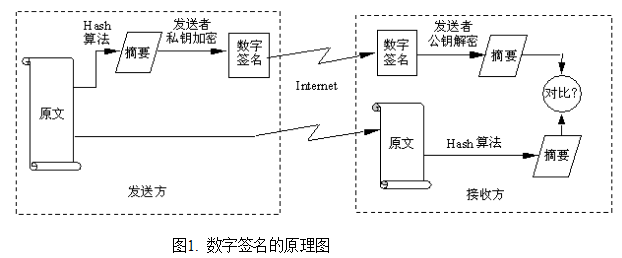
\includegraphics[width=0.7\linewidth]{dsa.png}
	\end{figure}
	\begin{enumerate}
		\item 使用SHA编码将发送文件加密产生128bit的数字摘要; 
		\item 发送方用自己的专用密钥对摘要再加密,形成数字签名; 
		\item 将原文和加密的摘要同时传给对方; 
		\item 接受方用发送方的公共密钥对摘要解密,同时对收到的文件用SHA编码加密产生同一摘要; 
		\item 将解密后的摘要和收到的文件在接受方重新加密产生的摘要相互对比,如果两者一致,则说明在传送过程中信息没有破坏和篡改。否则,则说明信息已经失去安全性和保密性。
	\end{enumerate}
	\item RSA
	签名方产生一对公钥(N,e)和私钥(N,d)之后,就可以对消息进行签名。
	\begin{enumerate}
		\item 利用摘要算法计算消息的摘要H(M)
		\item 用私有密钥(n,d)加密消息摘要得到$ s = H(M)^d  mod  n $
		\item 签名完成后,签名房将(M,s)发送给对方
		\item 接收方利用摘要算法计算消息的摘要$ H(M_1) $
		\item 再用公开密钥(n,e)解密消息摘要得到$ s1 = s^e  mod n $,比对$ s1 = H(M_1) $,如果相同则通过,否则拒绝接受。
	\end{enumerate}
\end{enumerate}


\question{消息认证} 值接收方对收到的消息进行检验,检验内容包括消息的源地址、目的地址,消息的内容是否收到篡改以及消息的有效生存时间等。消息认证可以时实时的也可以是非实时的。\\
消息认证离不开HASH函数。这里介绍几个概念:
\begin{enumerate}
	\item 单向函数,已知$ x $计算$ y=f(x) $很容易,但是已知$ y $很难求出$ x = f^{-1}(x) $
	\item 哈希函数,将\textbf{可变长度}的输入映射为\textbf{固定长度},同时不同输入应该有不同输出。哈希函数不一定是单向函数,即是哈希又是单向的成为\textbf{单向哈希函数}
	\item 单向陷门函数,特殊的单向函数,在不知道秘密陷门时,很难反向计算,但是知道了秘密陷门,很容易计算反向函数。
\end{enumerate}
消息认证的方式有两种
\begin{enumerate}
	\item 采用消息认证码,需要密钥参与
	\item 采用Hash函数,不需要密钥参与。将任意长度消息M映射为一个较小固定长度值H(M)。原消息中任何一个bit的改变都会使得Hash码发生巨大改变。因此可以利用Hash函数检测消息传播过程中\textbf{是否遭受篡改}(类似于CRC)。配置\textbf{非对称加密算法(如DSA,RSA)}可进行数字签名的功能。
\end{enumerate}  

\question{消息认证算法}
\begin{description}
	\item[MD5] 输入任意长,以512位为单位分成快,输出是128为的消息摘要。步骤
	\begin{enumerate}
		\item 填充字节,增加的长度在1-512.从而使填充后的消息长度为$ 512n-64 $。64用来记录消息长度。
		\item 分块,每块长度512
		\item 初始化寄存器
		\item 处理每一个分块,由压缩函数处理
		\item 输出结果
	\end{enumerate}
	用处:
	\begin{enumerate}
		\item 防止被篡改
		\item 防止直接看到明文
		\item 防止抵赖(数字签名)
	\end{enumerate}
	\item SHA算法,输入上限$ 2^64 $,输出160.算法流程和MD5相同。但是在“处理每一个分块”时,压缩函数迭代次数更多。
	\item HMAC算法,SSL中使用了HMAC算法。
\end{description}

\question{身份认证的概念} 目的是在不可信的网络上建立通信实体之间的信任关系。有
\begin{enumerate}
	\item 口令认证
	\item 智能卡认证
	\item 基于生物特征的认证
	\item 双因素认证
	\item 基于源地址的认证
	\item 基于PAP的认证
	\item 基于CHAP的认证
\end{enumerate}

\question{身份认证协议}
\begin{enumerate}
	\item 双向身份认证协议
	\item 单向身份认证协议
	\item 零知识身份认证协议
\end{enumerate}

\question{身份认证协议实例}
\begin{enumerate}
	\item RADIUS,远程身份验证拨入用户服务协议。用于\textbf{认证,计费,授权}
	\item Kerberos。通信主体客户A,服务器B以及认证服务器,票据服务器。
\end{enumerate}